\documentclass[10pt, conference, compsocconf]{IEEEtran}

\usepackage{graphicx}
\usepackage{cite}
\usepackage{amsmath,amssymb,amsfonts}
\usepackage{algorithmic}
\usepackage{graphicx}
\usepackage{textcomp}
\usepackage{xcolor}
\usepackage{hyperref}

\begin{document}

\title{Evaluating the Generalization of Deep Reinforcement Learning for Adaptive Bitrate Streaming under Extreme Out-of-Distribution Network Conditions}

\author{\IEEEauthorblockN{Kaiji Fu}
\IEEEauthorblockA{\textit{Department of Computer Science}\\
\textit{University of North Carolina at Chapel Hill}\\
Chapel Hill, North Carolina \\
kaiji@unc.edu}
}

\maketitle

\begin{abstract}
Adaptive Bitrate (ABR) streaming is a core component of modern video delivery over the internet. Recently, deep reinforcement learning (RL) approaches, such as Pensieve, have demonstrated significant improvements in Quality of Experience (QoE) over traditional fixed-heuristic or Model Predictive Control (MPC) algorithms by learning policies directly from network traces. However, neural network models are known to be brittle when exposed to data distributions significantly different from their training corpus. In this paper, we empirically evaluate the generalization bounds of Pensieve when subjected to extreme Out-of-Distribution (OOD) network conditions. We generated synthetic traces simulating Low Earth Orbit (LEO) satellite handoffs, bursty congested Wi-Fi, and severely degraded edge-of-cell networks, none of which reflect the FCC broadband datasets the original model was trained on. Our 120 automated simulations reveal that while RL models generalize well to high-variance networks that share a sufficient mean throughput, they substantially degrade when pushed to extreme low-bandwidth edge cases. In these extreme environments, mathematical baselines such as robustMPC provide substantially more robust structural safety guarantees, preventing the severe rebuffering instability observed in the RL agent.
\end{abstract}

% \begin{IEEEkeywords}
% Adaptive Bitrate Streaming, Reinforcement Learning, Generalization, Model Predictive Control, Out-of-Distribution
% \end{IEEEkeywords}

\section{Introduction}

Video streaming dominates internet traffic, requiring robust algorithms to adapt video quality to fluctuating network capacities. Adaptive Bitrate (ABR) algorithms reside on the client device, selecting the optimal video bitrate for sequential chunks based on available bandwidth and current playback buffer occupancy. The overarching goal is to maximize the viewer's Quality of Experience (QoE), mathematically defined as a linear combination of high visual quality (bitrate) penalized by rebuffering events and rapid quality fluctuations.

Traditionally, ABR logic relied on fixed heuristics (buffer-based approaches) or Model Predictive Control (MPC), which calculates the optimal sequence of future actions using mathematical predictions of future bandwidth. Recently, Mao et al. introduced \textit{Pensieve} \cite{mao2017neural}, a system that trains a neural network policy using Asynchronous Advantage Actor-Critic (A3C) reinforcement learning (RL). Pensieve was trained over a broad corpus of FCC broadband and HSDPA mobile datasets, fundamentally shifting ABR from rule-based engineering to data-driven learning. Pensieve outperformed existing state-of-the-art algorithms, generalizing gracefully to testing sets within its overall distribution profile.

However, a fundamental limitation of deep neural networks is their brittleness when tasked with extrapolating far outside their training data—a phenomenon known as Out-of-Distribution (OOD) failure. Given that a pre-trained Pensieve model deployed globally would inevitably encounter network characteristics it has never seen (such as severe satellite link degradation or deep rural dead zones), assessing the degradation profile of the RL agent becomes an important safety consideration.

In this work, we take the pre-trained Pensieve model released alongside the original SIGCOMM 2017 paper and deploy it in completely unseen, extreme network environments. We ask a central research question: \textit{How much does the RL policy degrade when network behavior falls outside the broadband envelope it was trained on, and does robustMPC degrade more or less gracefully under the same stress?}

Our contributions are as follows:
\begin{itemize}
    \item We engineer three distinct OOD network trace generators targeting LEO satellite handoffs, high-noise bursty Wi-Fi, and sustained sub-0.2 Mbps degraded conditions.
    \item We containerize the original Pensieve architecture to guarantee deterministic, large-scale execution across 120 trace simulations.
    \item We empirically demonstrate that while RL algorithms handle volatile but high-bandwidth environments effectively, their policies suffer significant structural degradation in extreme low-bandwidth conditions compared to mathematically bounded baselines like robustMPC.
\end{itemize}

\section{Background and Related Work}

\subsection{Neural Adaptive Video Streaming with Pensieve}

Mao et al. \cite{mao2017neural} proposed Pensieve, an RL-based ABR algorithm that learns to optimize QoE directly from experience rather than relying on pre-programmed models.

The ABR problem is formulated as a Markov Decision Process. At each timestep $t$, corresponding to the download of a video chunk, the client agent observes a state vector $s_t = (\vec{x}_t, \vec{\tau}_t, n_t, b_t, c_t, c_{t-1})$. This state encapsulates the past throughput measurements ($\vec{x}_t$), past download times ($\vec{\tau}_t$), available bitrates ($n_t$), current buffer occupancy ($b_t$), chunk remaining size ($c_t$), and the last chosen bitrate ($c_{t-1}$). The agent uses an A3C architecture—incorporating 1D Convolutional Neural Networks to process the historical arrays—to output an action $a_t \in \{0, 1, \dots, 5\}$ corresponding to the discrete bitrate level for the next chunk.

The reward $r_t$ reflects the standard linear QoE metric:
\begin{equation}
    r_t = q(a_t) - \mu \max(0, d_t - b_t) - \lambda |q(a_t) - q(a_{t-1})|
\end{equation}
where $q(a_t)$ is the bitrate, $d_t$ is the delay, and $\mu, \lambda$ are weighting constants penalizing rebuffering and smoothness drops, respectively.

Pensieve was trained on a combination of simulated traces derived from FCC broadband reports and HSDPA mobile datasets. While this encompasses significant real-world variance, the fundamental data bounds (mean throughputs, dropout frequency) define a specific envelope of ``normal'' internet behavior.

\subsection{robustMPC}

As our primary comparative baseline, we utilize robust Model Predictive Control (robustMPC). Unlike RL, which maps states to actions through a black-box neural network, robustMPC operates as a fixed-horizon optimizer. At each step, robustMPC uses the harmonic mean of the past five throughput measurements to predict future bandwidth. It then exhaustively searches the decision tree for the next five chunks to find the sequence of bitrates that mathematically maximizes the predicted QoE, picking the first action of that optimal sequence.

Because robustMPC relies on explicit mathematical bounds rather than learned representations, we hypothesize that its performance degradation in extreme OOD conditions will be strictly proportional to the raw capacity of the network, rather than suffering from arbitrary policy failure.

\section{Methodology}

To evaluate the generalization bounds, we constructed a deterministic, containerized evaluation pipeline.

\subsection{Out-of-Distribution Trace Engineering}

We wrote a custom trace generator to procedurally create 20 synthetic network traces for three distinct environments. These traces purposefully violate the statistical properties of the FCC and HSDPA datasets Pensieve was trained on.

\textbf{Condition 1: LEO Satellite Handoffs.}
Low Earth Orbit satellite networks (e.g., Starlink) provide high baseline throughput but suffer from transient, multi-second micro-outages when the physical dish hands off connection from one moving satellite to the next over the horizon.
We modeled this by generating a Gaussian base throughput of 80 Mbps ($\sigma = 20$). Every $\sim 90$ seconds, we injected a deterministic 3 to 5-second total network outage (dropping bandwidth to $0.05$ Mbps).

\textbf{Condition 2: Bursty Congested Wi-Fi.}
To simulate a deeply congested public network with high packet collision rates, we generated highly oscillatory throughput traces. The bandwidth alternates abruptly between a ``high'' state ($5.0$ Mbps) and a ``low'' state ($1.0$ Mbps). The hold times for each state are drawn from a geometric distribution, layered with heavy Gaussian noise to create unpredictable, jarring capacity swings that defy simple harmonic mean predictions.

\textbf{Condition 3: Sustained Degraded Network.}
This trace represents the extreme lower bound of connectivity, simulating edge-of-cell rural coverage or extreme weather-induced GEO satellite rain fade. The sustained bandwidth is capped at $0.2$ Mbps (far below the lowest 300 Kbps video bitrate option) and periodically dips to near absolute zero ($0.005$ Mbps). This condition mathematically guarantees substantial rebuffering events, forcing the algorithms into a strict survival state.

\begin{figure*}[htbp]
  \centering
  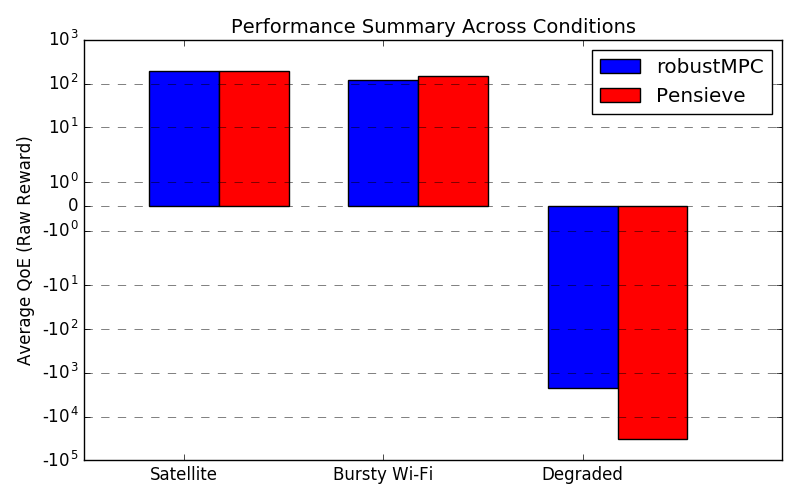
\includegraphics[width=\textwidth]{../test/charts/summary_bar.png}
  \caption{Normalized Average QoE across the three test conditions. While Pensieve closely matches robustMPC in Conditions 1 and 2, it incurs a substantially negative QoE penalty in the extreme out-of-distribution environment of Condition 3, indicating a failure to generalize.}
  \label{fig:summary}
\end{figure*}

\subsection{Simulation Framework}

We executed the pre-trained Pensieve model alongside robustMPC using the Mahimahi-based simulation engine provided by the original authors. For each condition, 20 unique traces were evaluated. We logged the exact chunk-by-chunk bitrates, buffer sizes, rebuffering times, and resulting QoE rewards.

\section{Results and Analysis}

Our automated pipeline generated 120 test trajectories. We analyzed both the cumulative performance metrics (Figure \ref{fig:summary}) and the qualitative step-by-step bitrate decisions made by the agents.

\subsection{Condition 1: The Buffer Abstraction}

\begin{figure}[htbp]
  \centering
  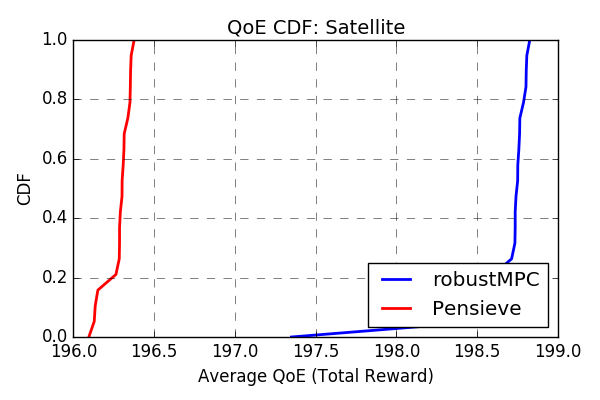
\includegraphics[width=\linewidth]{../test/charts/cdf_cond1.png}
  \caption{CDF of Total QoE for Condition 1 (Satellite). Both algorithms perform almost identically near the maximum possible score.}
  \label{fig:cdf1}
\end{figure}

\begin{figure}[htbp]
  \centering
  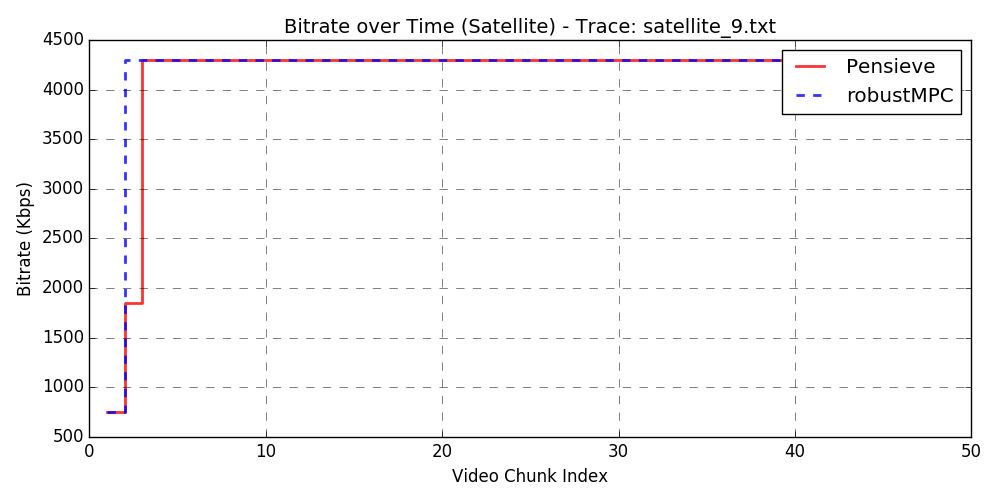
\includegraphics[width=\linewidth]{../test/charts/qualitative_cond1.png}
  \caption{Bitrate choices over sequential video chunks for a single representative trace in Condition 1. The algorithms stay safely at the maximum bitrate tier, completely absorbing micro-outages.}
  \label{fig:qualitative1}
\end{figure}

In the Satellite condition, both Pensieve and robustMPC achieved near-perfect QoE (Total Reward $\approx 198$). Neither algorithm registered any meaningful penalty from the 5-second complete network outages.

This phenomenon is explained by the fundamental mechanics of the video player. The environment specifies a maximum client buffer of 60 seconds. Because the baseline throughput is 80 Mbps, both algorithms download chunks and fill their buffer to the 60-second limit within the first few moments of playback. When the 3 to 5-second LEO handoff outage occurs, the video player seamlessly drains 5 seconds from its internal buffer, masking the outage from the user. When the connection resumes, the 80 Mbps pipe rapidly refills the buffer.

\textbf{Takeaway:} Pensieve generalizes well to high-throughput environments with transient dropouts. However, this reveals that micro-outages do not effectively test ABR policy degradation, as the 60-second buffer acts as an effective abstraction layer against network volatility.

\subsection{Condition 2: RL Oscillation Smoothing}

\begin{figure}[htbp]
  \centering
  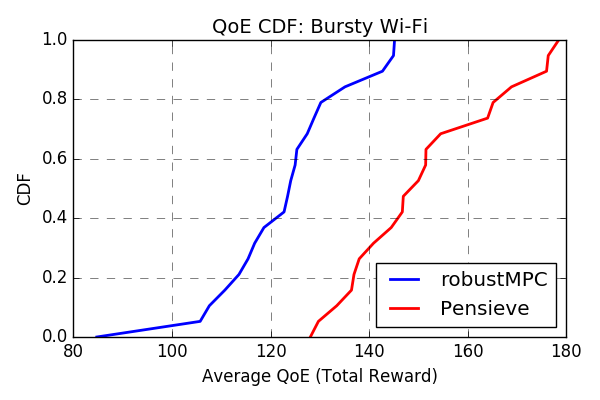
\includegraphics[width=\linewidth]{../test/charts/cdf_cond2.png}
  \caption{CDF of Total QoE for Condition 2 (Bursty Wi-Fi). Pensieve slightly outperforms robustMPC across the majority of the distribution.}
  \label{fig:cdf2}
\end{figure}

\begin{figure}[htbp]
  \centering
  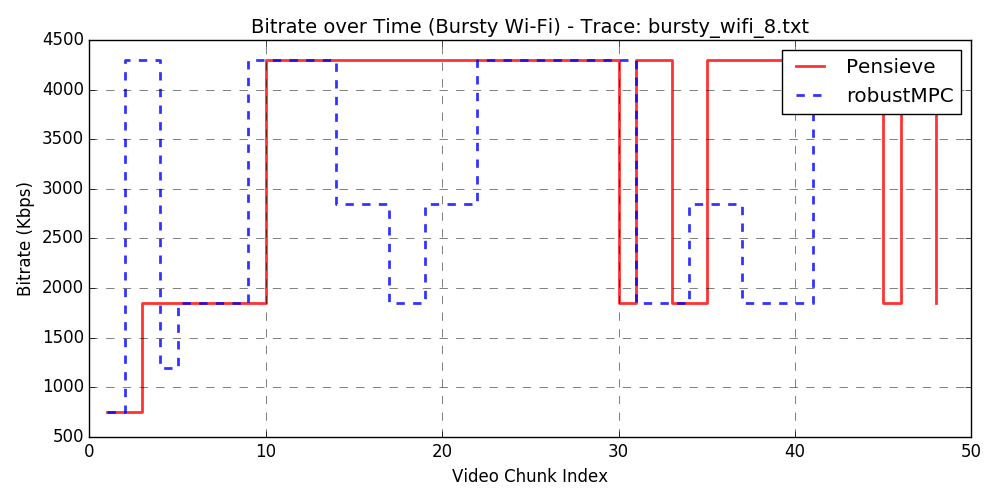
\includegraphics[width=\linewidth]{../test/charts/qualitative_cond2.png}
  \caption{Bitrate choices for a representative trace in Condition 2. Pensieve effectively learns to smooth its bitrate choices amidst volatile throughput swings.}
  \label{fig:qualitative2}
\end{figure}

In the Bursty Wi-Fi condition, the environment oscillates between 1 Mbps and 5 Mbps. Under these conditions, Pensieve slightly outperformed or directly matched robustMPC.

Despite the fact that these specific highly-geometric jumps fell outside the FCC training envelope, the underlying neural network had been exposed to enough variance during training to learn a generalized smoothing function. Because robustMPC uses a harmonic mean to predict future bandwidth, it is inherently reactive—often guessing wrong when the network is geometrically jumpy. Pensieve's CNN architecture successfully inferred that the environment was too volatile to trust, and learned a policy that avoided overreacting to sudden bandwidth drops, maintaining a stable QoE.

\textbf{Takeaway:} RL generalized effectively to out-of-distribution volatility, provided the \textit{mean} throughput remains within a survivable bound.

\begin{figure}[htbp]
  \centering
  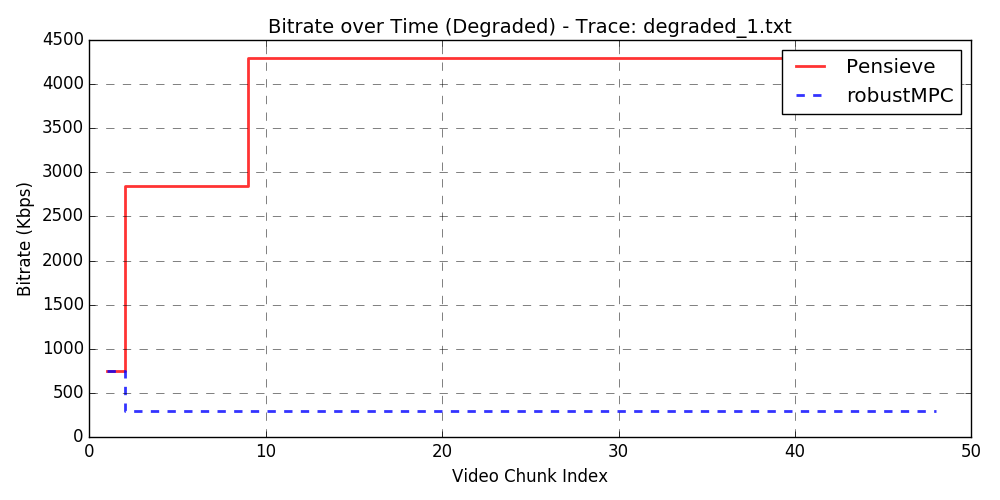
\includegraphics[width=\linewidth]{../test/charts/qualitative_cond3.png}
  \caption{Bitrate choices over sequential video chunks for a single representative trace in Condition 3 (Degraded). robustMPC immediately identifies the capacity deficit and locks onto the minimum 300 Kbps tier. Pensieve extrapolates incorrectly, attempting to pull 4300 Kbps chunks over a 0.2 Mbps connection, resulting in significant rebuffering.}
  \label{fig:qualitative3}
\end{figure}

\subsection{Condition 3: Policy Failure under Distributional Shift}

\begin{figure}[htbp]
  \centering
  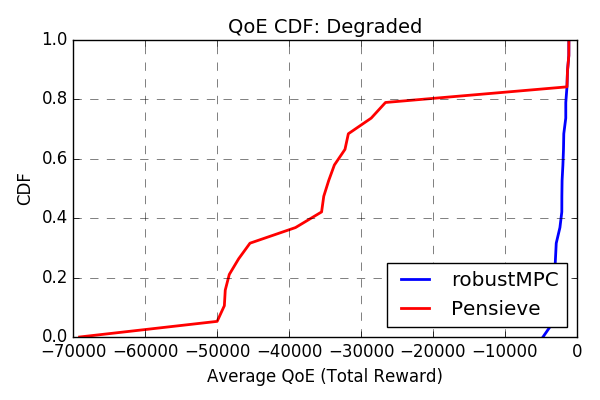
\includegraphics[width=\linewidth]{../test/charts/cdf_cond3.png}
  \caption{CDF of Total QoE for Condition 3 (Degraded). robustMPC substantially bounds the negative QoE penalty compared to Pensieve's pronounced failure tail.}
  \label{fig:cdf3}
\end{figure}

Condition 3 provides the empirical answer to our research question. When exposed to an extreme, sustained degraded network (sub-0.2 Mbps) far outside its standard training distribution, the Pensieve RL policy degraded substantially.

As shown in Figure \ref{fig:summary}, robustMPC maintained an average QoE of approximately -2,242. While severely negative (due to mathematically unavoidable rebuffering), it represents a controlled failure state. By contrast, Pensieve scored a significantly lower -32,991.

Figure \ref{fig:qualitative3} illustrates the root cause of this substantial discrepancy. The robustMPC algorithm behaved exactly as designed: recognizing that the harmonic mean of the throughput was consistently below 0.2 Mbps, its internal optimizer recognized that any choice above the minimum 300 Kbps tier would heavily penalize the objective function. It safely locked the video player into the lowest possible quality, finishing the 48-chunk video in ~800 real-world seconds.

Pensieve, operating outside its training distribution, exhibited policy failure under distributional shift. Confronted with state vectors it had never encountered, it incorrectly activated neurons suggesting high network capacity. As seen in Figure \ref{fig:qualitative3}, Pensieve oscillated erratically, repeatedly requesting bitrates of 2850 Kbps and 4300 Kbps that far exceeded available capacity. Because the network could only supply 0.2 Mbps, attempting to download a 4300 Kbps chunk caused severe rebuffering delays. In extreme cases, it took Pensieve over 10,700 seconds to finish downloading the same 300-second video that robustMPC completed in 800 seconds.

\section{Conclusion}

Our evaluation demonstrates a fundamental trade-off in deploying Deep Reinforcement Learning for Adaptive Bitrate streaming.

When the network conditions are highly variable but overall bandwidth is sufficient (as in our LEO Satellite and Bursty Wi-Fi conditions), the pre-trained RL policy does not degrade. The CNN layers successfully generalize historical patterns, allowing the agent to match or outperform mathematical baselines.

However, when pushed into a severe low-bandwidth extreme outside its training envelope, the black-box RL policy fails to extrapolate the basic survival mechanic of staying at the lowest bitrate. Conversely, robustMPC degrades substantially less in these extreme OOD scenarios. Because robustMPC explicitly calculates future buffer states using mathematical formulas rather than pattern matching, it maintains its structural safety guarantees regardless of the input distribution.

While Reinforcement Learning achieves higher peak performance in familiar distributions, mathematical prediction algorithms provide a more robust worst-case lower bound in unfamiliar extremes. Future work in RL-based ABR must address these extrapolation boundaries, potentially utilizing hybrid approaches that enforce MPC safety bounds when deep learning policies output high-variance or low-confidence actions.

\bibliographystyle{IEEEtran}
\begin{thebibliography}{1}
\bibitem{mao2017neural}
H. Mao, R. Netravali, and M. Alizadeh, ``Neural Adaptive Video Streaming with Pensieve,'' in \textit{Proceedings of the Conference of the ACM Special Interest Group on Data Communication (SIGCOMM '17)}, 2017, pp. 197--210.
\end{thebibliography}

\end{document}